\documentclass[hidelinks,12pt]{article}
\usepackage[left=0.25cm,top=1cm,right=0.25cm,bottom=1cm]{geometry}
%\usepackage[landscape]{geometry}
\textwidth = 20cm
\hoffset = -1cm
\usepackage[utf8]{inputenc}
\usepackage[spanish,es-tabla, es-lcroman]{babel}
\usepackage[autostyle,spanish=mexican]{csquotes}
\usepackage[tbtags]{amsmath}
\usepackage{nccmath}
\usepackage{amsthm}
\usepackage{amssymb}
\usepackage{mathrsfs}
\usepackage{graphicx}
\usepackage{subfig}
\usepackage{caption}
%\usepackage{subcaption}
\usepackage{standalone}
\usepackage[outdir=./Imagenes/]{epstopdf}
\usepackage{siunitx}
\usepackage{physics}
\usepackage{color}
\usepackage{float}
\usepackage{hyperref}
\usepackage{multicol}
\usepackage{multirow}
%\usepackage{milista}
\usepackage{anyfontsize}
\usepackage{anysize}
%\usepackage{enumerate}
\usepackage[shortlabels]{enumitem}
\usepackage{capt-of}
\usepackage{bm}
\usepackage{mdframed}
\usepackage{relsize}
\usepackage{placeins}
\usepackage{empheq}
\usepackage{cancel}
\usepackage{pdfpages}
\usepackage{wrapfig}
\usepackage[flushleft]{threeparttable}
\usepackage{makecell}
\usepackage{fancyhdr}
\usepackage{tikz}
\usepackage{bigints}
\usepackage{menukeys}
\usepackage{tcolorbox}
\tcbuselibrary{breakable}
\usepackage{scalerel}
\usepackage{pgfplots}
\usepackage{pdflscape}
\pgfplotsset{compat=1.16}
\spanishdecimal{.}
\renewcommand{\baselinestretch}{1.5} 
\renewcommand\labelenumii{\theenumi.{\arabic{enumii}})}

\newcommand{\python}{\texttt{python}}
\newcommand{\textoazul}[1]{\textcolor{blue}{#1}}
\newcommand{\azulfuerte}[1]{\textcolor{blue}{\textbf{#1}}}
\newcommand{\funcionazul}[1]{\textcolor{blue}{\textbf{\texttt{#1}}}}

\newcommand{\pderivada}[1]{\ensuremath{{#1}^{\prime}}}
\newcommand{\sderivada}[1]{\ensuremath{{#1}^{\prime \prime}}}
\newcommand{\tderivada}[1]{\ensuremath{{#1}^{\prime \prime \prime}}}
\newcommand{\nderivada}[2]{\ensuremath{{#1}^{(#2)}}}


\newtheorem{defi}{{\it Definición}}[section]
\newtheorem{teo}{{\it Teorema}}[section]
\newtheorem{ejemplo}{{\it Ejemplo}}[section]
\newtheorem{propiedad}{{\it Propiedad}}[section]
\newtheorem{lema}{{\it Lema}}[section]
\newtheorem{cor}{Corolario}
\newtheorem{ejer}{Ejercicio}[section]

\newlist{milista}{enumerate}{2}
\setlist[milista,1]{label=\arabic*)}
\setlist[milista,2]{label=\arabic{milistai}.\arabic*)}
\newlength{\depthofsumsign}
\setlength{\depthofsumsign}{\depthof{$\sum$}}
\newcommand{\nsum}[1][1.4]{% only for \displaystyle
    \mathop{%
        \raisebox
            {-#1\depthofsumsign+1\depthofsumsign}
            {\scalebox
                {#1}
                {$\displaystyle\sum$}%
            }
    }
}
\def\scaleint#1{\vcenter{\hbox{\scaleto[3ex]{\displaystyle\int}{#1}}}}
\def\scaleoint#1{\vcenter{\hbox{\scaleto[3ex]{\displaystyle\oint}{#1}}}}
\def\scaleiiint#1{\vcenter{\hbox{\scaleto[3ex]{\displaystyle\iiint}{#1}}}}
\def\bs{\mkern-12mu}

\newcommand{\Cancel}[2][black]{{\color{#1}\cancel{\color{black}#2}}}


\usepackage{minted}
\usetikzlibrary{arrows, arrows.meta}

\title{\vspace{-2cm} El método de Ridder \\ {\large Material de apoyo Búsqueda de raíces} \vspace{-3ex}}
\author{M. en C. Gustavo Contreras Mayén. \texttt{gux7avo@ciencias.unam.mx}}
\date{}

\begin{document}

\fontsize{14}{14}\selectfont
\vspace{-4cm}
\maketitle

\section{Definición.}

El  \textbf{método de Ridder} es una modificación inteligente del \emph{método de la falsa posición}, veamos cómo se construye.
\par
Suponiendo que la raíz está entre paréntesis $(x_{1}, x_{2})$, primero calculamos $f_{3} = f (x_{3})$, donde $x_{3}$ es el punto medio del paréntesis, como se indica en la figura (\ref{fig:figura_04_03a}).
\begin{figure}[H]
    \centering
    \begin{tikzpicture}
        \draw (0, 0) -- (7, 0) node [above, near end, pos=1] {$x$};
        \draw (0, 0) -- (0, 2) node [left, near end, pos=1] {$ f (x)$};
        \draw [thick] (1, 1.3) .. controls (3, 0.6) .. (5.5, -1);
        \draw (1.3, 1.2) circle (2pt);
        \draw (3, 0.54) circle (2pt);
        \draw (4.7, -0.5) circle (2pt);
        \node at (1.6, -0.3) {$x_{1}$};
        \node at (3.3, -0.3) {$x_{3}$};
        \node at (5, 0.3) {$x_{2}$};
        \draw [dashed] (1.3, 0) -- (1.3, 1.2);
        \draw [dashed] (3, 0) -- (3, 0.54);
        \draw [dashed] (4.7, 0) -- (4.7, -0.5);
        \draw (1.3, 0) -- (1.3, -1);
        \draw (3, 0) -- (3, -1);
        \draw (4.7, -0.5) -- (4.7, -1);
        \draw [stealth-stealth, thick] (1.3, -0.8) -- (3, -0.8) node [below, midway] {$h$};
        \draw [stealth-stealth, thick] (3, -0.8) -- (4.7, -0.8) node [below, midway] {$h$};
    \end{tikzpicture}
    \caption{Construyendo el método de Ridder}
    \label{fig:figura_04_03a}
\end{figure}

A continuación introducimos la función:
\begin{align}
g (x) = f (x) \, \exp\big( (x - x_{1}) \, Q \big)
\label{eq:ecuacion_a} 
\end{align}
donde la constante $Q$ se determina haciendo que los puntos $(x_{1}, g_{1})$, $(x_{2}, g_{2})$ y $(x_{3}, g_{3})$ estén en línea recta, como se muestra en la figura ().
\begin{figure}[H]
    \centering
    \begin{tikzpicture}
        \draw (0, 0) -- (7, 0) node [above, near end, pos=1] {$x$};
        \draw (0, 0) -- (0, 2) node [left, near end, pos=1] {$ g (x)$};
        \draw [thick] (1, 1.3) -- (5.5, -1);
        \draw (1.3, 1.2) circle (2pt);
        \draw (3, 0.3) circle (2pt);
        \draw (3.5, 0) circle (2pt);
        \draw (4.7, -0.6) circle (2pt);
        \node at (1.6, -0.3) {$x_{1}$};
        \node at (2.7, -0.3) {$x_{3}$};
        \node at (3.6, 0.3) {$x_{4}$};

        \node at (5, 0.3) {$x_{2}$};
        \draw [dashed] (1.3, 0) -- (1.3, 1.2);
        \draw [dashed] (3, 0) -- (3, 0.3);
        \draw [dashed] (4.7, 0) -- (4.7, -0.5);
        \draw (1.3, 0) -- (1.3, -1);
        \draw (3, 0) -- (3, -1);
        \draw (4.7, -0.5) -- (4.7, -1);
        \draw [stealth-stealth, thick] (1.3, -0.8) -- (3, -0.8) node [below, midway] {$h$};
        \draw [stealth-stealth, thick] (3, -0.8) -- (4.7, -0.8) node [below, midway] {$h$};
    \end{tikzpicture}
    \caption{Construyendo el método de Ridder}
    \label{fig:figura_04_03b}
\end{figure}

Como antes, la notación que usamos es $g_{i} = g (x_{i})$. El valor mejorado de la raíz se obtiene luego por interpolación lineal de $g (x)$ en lugar de $f (x)$.
\par
Veamos ahora los detalles. De la ecuación. (\ref{eq:ecuacion_a}) obtenemos:
\begin{align}
g_{1} = f_{1} \hspace{1.3cm} g_{2} = f_{2} \, \exp(2 \, h \, Q) \hspace{1.3cm} g_{3} = f_{3} \, \exp(h \, Q)
\label{eq:ecuacion_b}
\end{align}
donde $h = (x_{2} - x_{1}/2)$.
\par
El requisito de que los tres puntos de la figura (\ref{fig:figura_04_03b}) estén sobre una línea recta es $g_{3} = ( g_{1} + g_{2})/2$, o:
\begin{align*}
f_{3} \, \exp(h \, Q) = \dfrac{1}{2} \bigg[ f_{1} + f_{2} \exp(2 \, h \, Q) \bigg]
\end{align*}
que es una ecuación cuadrática en $\exp(h \, Q)$. La solución es:
\begin{align}
\exp(h \, Q) = \dfrac{f_{3} \pm \sqrt{f_{3}^{2} - f_{1} \, f_{2}}}{f_{2}}
\label{eq:ecuacion_c}
\end{align}
La interpolación lineal basada en los puntos $(x_{1}, g_{1})$ y $(x_{3}, g_{3})$ ahora da como resultado la raíz mejorada:
\begin{align*}
x_{4} &= x_{3} - g_{3} \, \dfrac{x_{3} - x_{1}}{g_{3} - g_{1}} = \\
&= x_{3} - f_{3} \, \exp(h \, Q) \, \dfrac{x_{3} - x_{1}}{f_{3} \, \exp(h \, Q) - f_{1}}
\end{align*}
donde en el último paso usamos las ecs. (\ref{eq:ecuacion_b}). Como paso final, sustituimos $\exp(h \, Q)$ de la ec. (\ref{eq:ecuacion_c}), y obtener después de un poco de álgebra:
\begin{align}
x_{4} = x_{3} \pm (x_{3} - x_{1}) \, \dfrac{f_{3}}{\sqrt{f_{3}^{2} - f_{1} \, f_{2}}}
\label{eq:ecuacion_04_03}
\end{align}
Se puede demostrar que el resultado correcto se obtiene eligiendo el signo más si $f_{1} - f_{2} > 0$, y el signo menos si $f_{1} - f_{2} < 0$. Después del cálculo de $x_{4}$, se determinan nuevos corchetes para la raíz y la ec. (\ref{eq:ecuacion_04_03}) se aplica de nuevo. El procedimiento se repite hasta que la diferencia entre dos valores sucesivos de $x_{4}$ se vuelve despreciable. La fórmula iterativa de Ridder en la ec. (\ref{eq:ecuacion_04_03}) tiene una propiedad muy útil: si $x_{1}$ y $x_{2}$ están a ambos lados de la raíz, entonces $x_{4}$ siempre está dentro del intervalo $(x_{1}, x_{2})$. En otras palabras, una vez que la raíz está entre corchetes, permanece entre corchetes, lo que hace que el método sea muy confiable. La desventaja es que cada iteración requiere dos evaluaciones de función. Hay métodos competitivos que se las arreglan con una sola evaluación de función por iteración, pero son más complejos y requieren un elaborado procedimiento.
\par
Se puede demostrar que el método de Ridder converge cuadráticamente, haciéndolo más rápido que el método de la secante o el de la falsa posición. Es el método a utilizar si la derivada de $f (x)$ es imposible o difícil de calcular.

\section{Ejercicios.}

\subsection{Ejercicio 1.}

Determina la raíz de:
\begin{align*}
f (x) = x^{3} - 10 \, x^{2} + 5 = 0
\end{align*}
que se encuentra en el intervalo $(0.6, 0.8)$ con el método de Ridder.
\par
\noindent
\textbf{Solución: } Para tener una idea de la función con la que estamos trabajando, hagamos un bosquejo que se presentamos en la gráfica (\ref{fig:figura_01}): 
\begin{figure}[H]
    \centering
    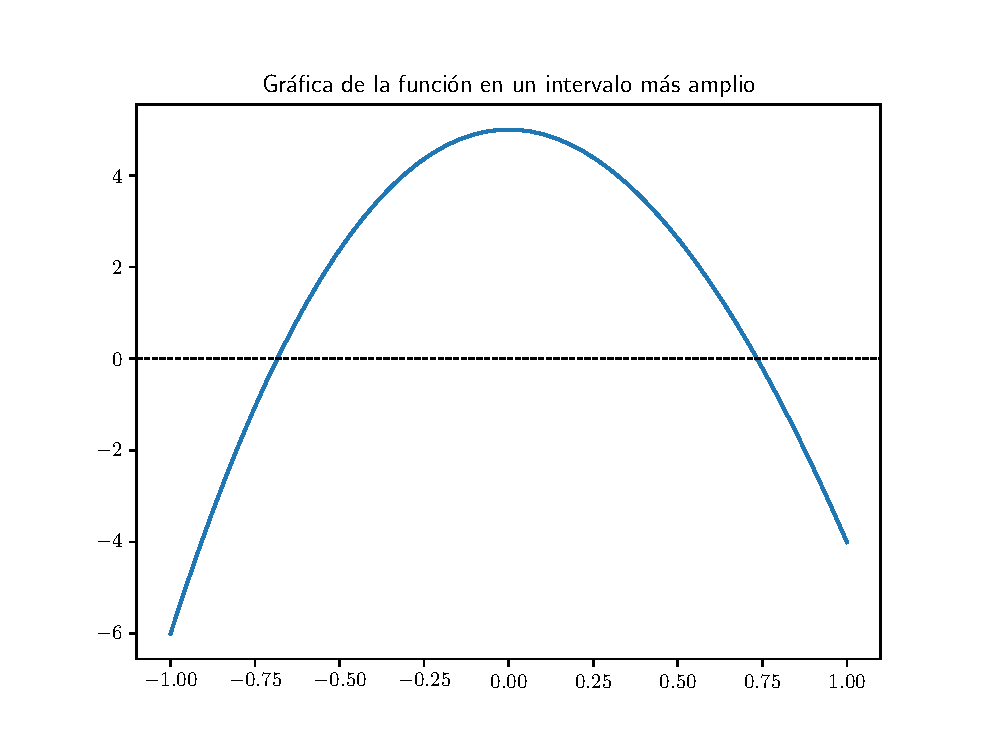
\includegraphics[scale=0.75]{Imagenes/plot_Metodo_Ridder_Ejercicio_01_01.eps}
    \caption{¿Tenemos un caso de raíz de duplicidad $2$?.}
    \label{fig:figura_01}
\end{figure}
Como el problema nos pide que calculemos la raíz en el intervalo $[0.6, 0.8]$, así que si hacemos un acercamiento a ese intervalo como se muestra en la figura (\ref{fig:figura_02}):
\begin{figure}[H]
    \centering
    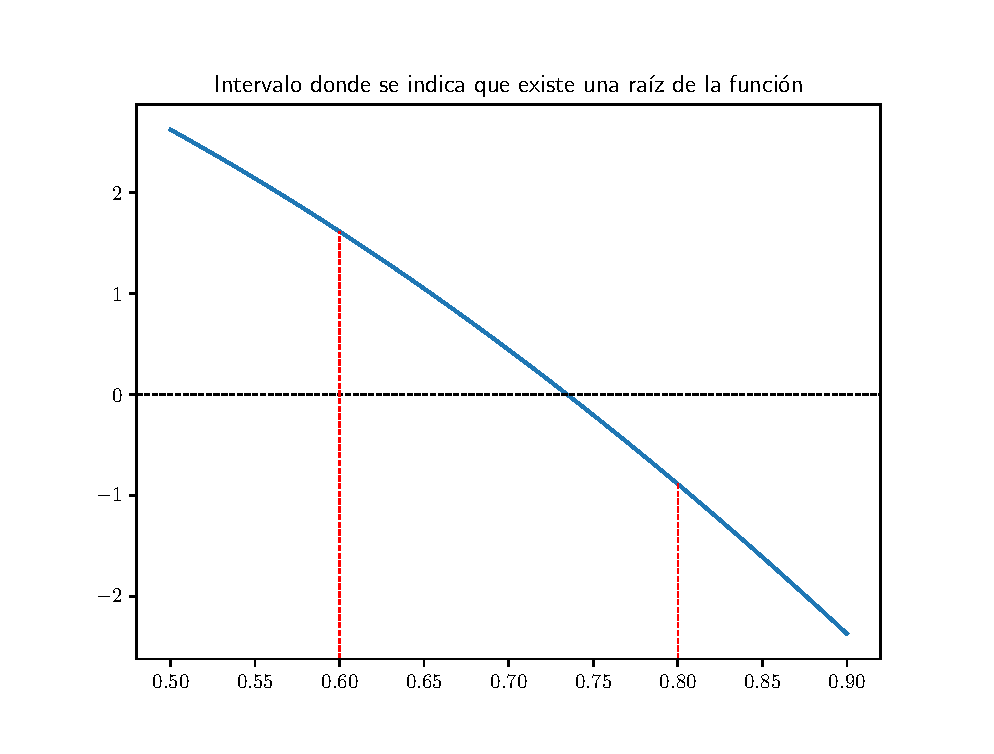
\includegraphics[scale=0.75]{Imagenes/plot_Metodo_Ridder_Ejercicio_01_02.eps}
    \caption{Acercamiento al intervalo de interés.}
    \label{fig:figura_02}
\end{figure}
Procedemos a ocupar la función \funcionazul{ridder} del módulo \funcionazul{metodoRidder}:
\begin{minted}{python}
from metodoRidder import ridder

x1 = 0.6
x2 = 0.8

raiz = ridder(f, x1, x2)
print('La raíz es: {0:1.4f}'.format(raiz))
\end{minted}

El resultado que se muestra en la terminal como:
\begin{minted}{python}
La raíz es: 0.7346 
\end{minted}
 En la figura (\ref{fig:figura_03}) se muestra la raíz de la función $f (x)$ en el intervalo $[0.6, 0.8]$.
\begin{figure}[H]
    \centering
    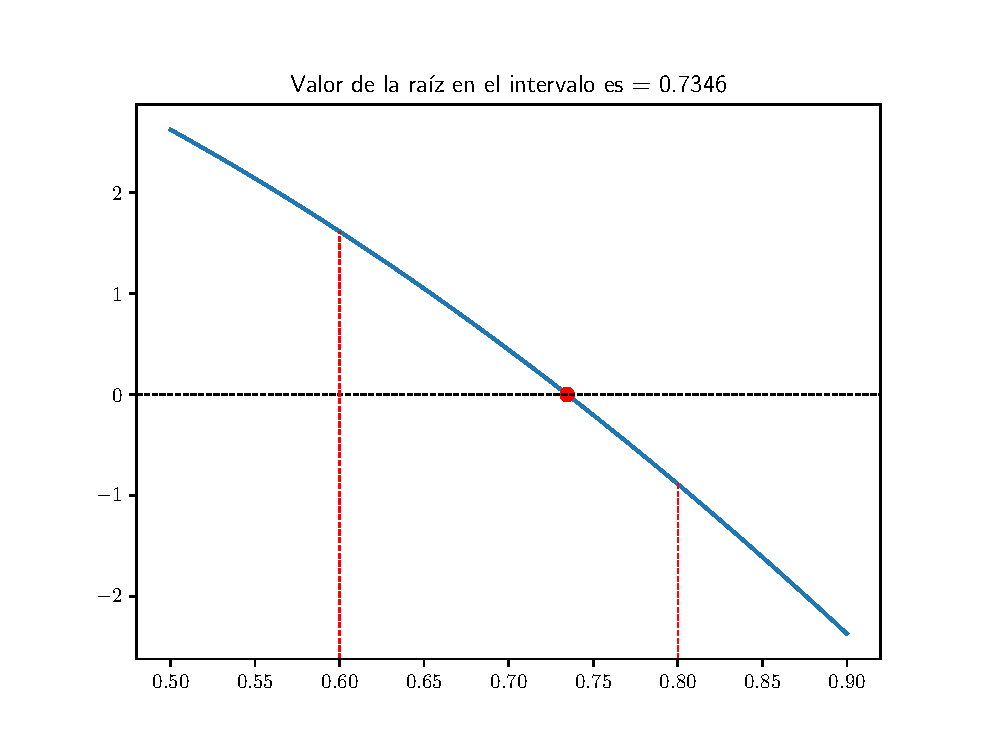
\includegraphics[scale=0.75]{Imagenes/plot_Metodo_Ridder_Ejercicio_01_03.eps}
    \caption{La raíz encontrada en el intervalo de interés.}
    \label{fig:figura_03}
\end{figure}

\subsection{Ejercicio 2.}

Calcula la raíz de la función:
\begin{align*}
f (x) = \dfrac{1}{(x - 0.3)^{2} + 0.01} - \dfrac{1}{(x - 0.8)^{2} + 0.04}
\end{align*}

En este ejercicio no se nos señala el intervalo en donde se encuentra la raíz, por lo que ocupamos nuestras habilidades de trabajo, para elaborar una gráfica de la función, que es la que se muestra como figura (\ref{fig:figura_04}):
\begin{figure}[H]
    \centering
    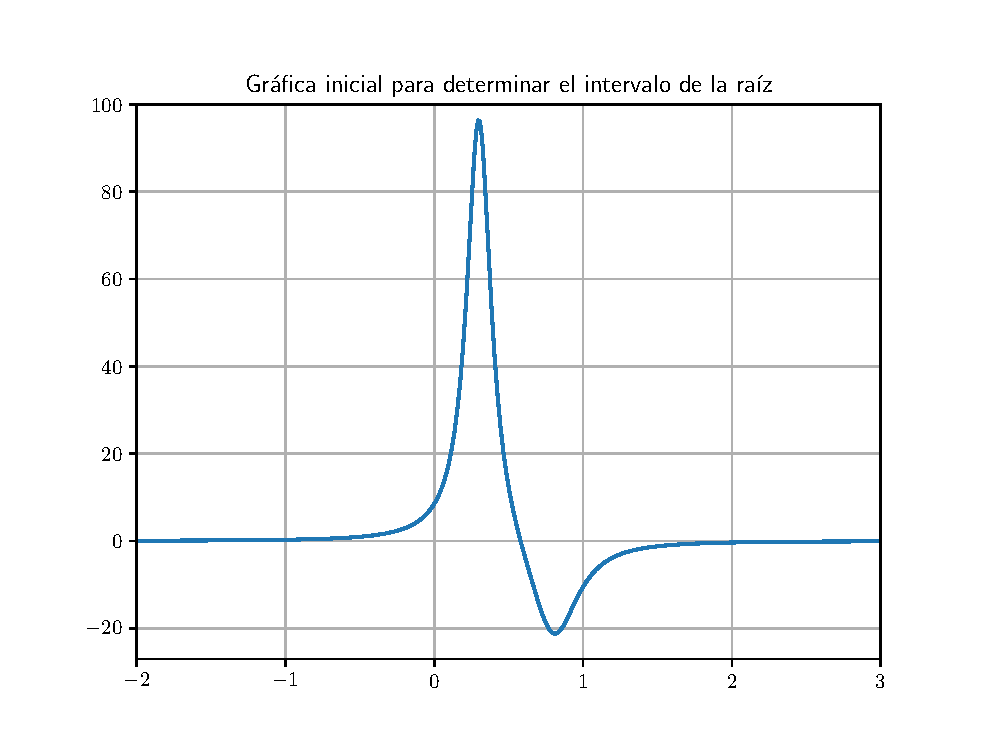
\includegraphics[scale=0.75]{Imagenes/plot_Metodo_Ridder_Ejercicio_02_01.eps}
    \caption{Gráfica de la función donde identificamos el intervalo de interés.}
    \label{fig:figura_04}
\end{figure}
De la figura anterior, vemos que de manera aproximada la raíz se encuentra entre $x = 0$ y $1$, por lo que ocupamos la función \funcionazul{ridder} en el siguiente código:
\begin{minted}{python}
from metodoRidder import ridder

def f(x):
    a = (x - 0.3)**2 + 0.01
    b = (x - 0.8)**2 + 0.04
    
    return 1./a - 1./b
  
raiz = ridder(f, 0., 1.)
print('La raíz es: {0:}'.format(raiz))
\end{minted}

El resultado de la raíz se presenta con la siguiente gráfica:
\begin{figure}[H]
    \centering
    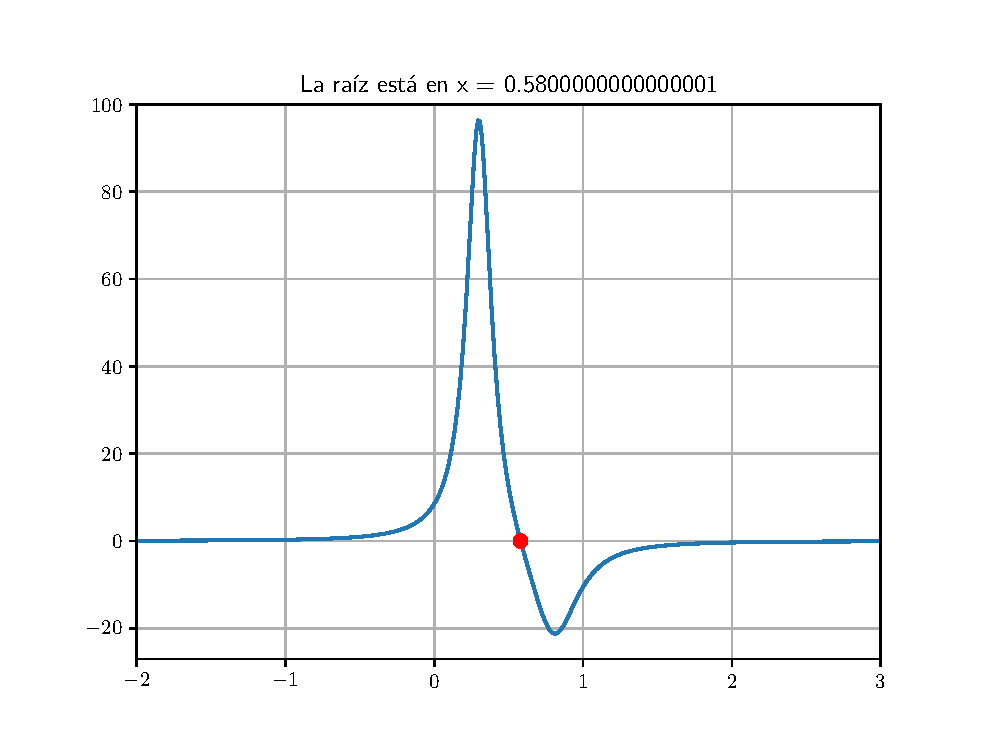
\includegraphics[scale=0.75]{Imagenes/plot_Metodo_Ridder_Ejercicio_02_02.eps}
    \caption{Gráfica con la raíz encontrada.}
    \label{fig:figura_05}
\end{figure}
Como habrás notado falta incluir las rutinas que generan las gráficas, pero que sin problema alguno puedes implementar y contar con el material completo de cada ejercicio.

\section{Resolviendo con funciones de python.}

En el módulo \funcionazul{scipy.optimize} se dispone de la función \funcionazul{ridder}, que ocupa el mencionado método de Ridder para calcular una raíz de la función $f$ entre los argumentos $a$ y $b$. Los argumentos mínimos son:
\begin{verbatim}
ridder(f, a, b)
\end{verbatim}
donde:
\begin{itemize}
\item \funcionazul{f}: Es una función continua y se requiere que $f (a)$ y $f (b)$ tengan signos contrarios.
\item \funcionazul{a}: Intervalo inicial para calcular la raíz.
\item \funcionazul{b}: Intervalo final para calcular la raíz.
\end{itemize}

La función \funcionazul{ridder} devuelve \funcionazul{$x_{0}$} que es el valor de la raíz de la función \funcionazul{f} definida en el intervalo \funcionazul{$[a, b]$}.
\par
En el siguiente ejemplo veremos la implementación de la función:

\begin{minted}{python}
from scipy.optimize import ridder

def f(x):
    return (x**2 - 1)
    
raiz1 = ridder(f, 0., 2.)
raiz2 = ridder(f, -2., 0.)
print('La raíz es: {0:}'.format(raiz1))
print('\nLa raíz es: {0:}'.format(raiz1))
\end{minted}
En la siguiente gráfica se muestra el resultado obtenido:
\begin{figure}[H]
    \centering
    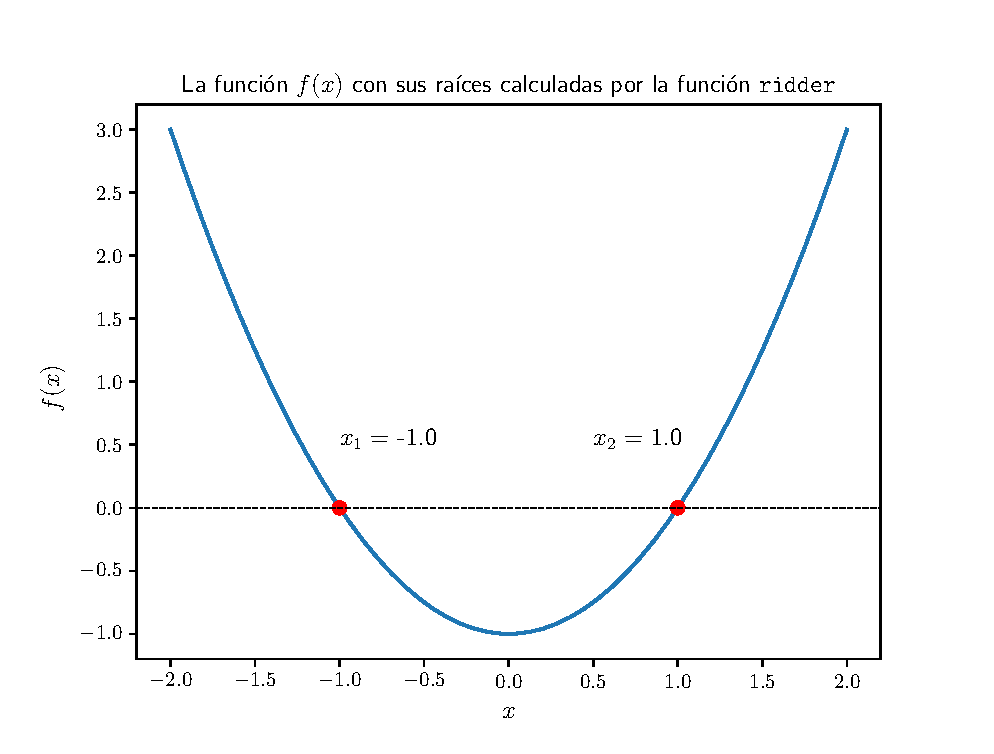
\includegraphics[scale=0.75]{Imagenes/plot_Metodo_Ridder_Ejercicio_03_01.eps}
    \caption{Gráfica con la raíz encontrada con la función \texttt{scipy.optimize.ridder}.}
    \label{fig:figura_06}
\end{figure}
\end{document}